\chapter{Hintergrundwissen}%
\label{cha:Hintergrundwissen}

\section{Konvexe Funktionen}%
\label{sec:Konvexe Funktionen}

\begin{definition}
\label{thm:konvexmenge}
	Eine Menge $X \subseteq \R^{n}$ heißt \underline{konvex} , wenn gilt
	\[
		\forall x,y \in X, \forall c \in [0,1] \colon 
		cx + (1-c)y \in X
	.\] 
\end{definition}

\begin{beispiel}
\label{thm:bspkonvexmenge}
Einige Beispiele

\begin{figure}[ht!]
	\begin{center}
		\includegraphics[width=0.5\textwidth]{pics/2.png}
	\end{center}
	\caption{Beispiele konvexer und nicht-konvexer Mengen}
	\label{fig:konvexemengen}
\end{figure}

\end{beispiel}

\begin{definition}
\label{thm:konvexfunktion}
	Sei $X \subseteq \R^{n}$ konvex. Dann heißt $f:X \rightarrow \R$
	\begin{enumerate}[label=\alph{enumi})]
		\item \underline{konvex} (auf $X$), wenn gilt
			\[
				\forall x,y \in X, \forall c \in [0,1] \colon f(cx + (1-c)y) \leq cf(x) + (1-c)f(y)
			.\] 
		\item \underline{strikt konvex} (auf $X$), wenn gilt
			\[
				\forall x,y \in X, x \neq y, \forall c \in (0,1) \colon f(cx + (1-c)y) < cf(x) + (1-c)f(y)
			.\] 
		\item \underline{gleichmäßig konvex} (auf $X$), wenn es ein $\mu>0$ gibt mit
			\[
				\forall x,y \in X, \forall c \in [0,1] \colon f(cx+ (1-c)y) \leq cf(x) + (1-c)f(y) - \mu c(1-c) \norm{x-y}^{2}
			.\] 
			\begin{figure}[ht!]
			\begin{center}
				\includegraphics[width=0.4\textwidth]{pics/texplot1.png} 
				\includegraphics[width=0.4\textwidth]{pics/texplot2.png}
			\end{center}
			\caption{links: konvexe Funktion, rechts: glm. konvexe Funktion}
			\label{fig:glmkonvexefunktion}
			\end{figure}

			Man kann Konvexität in einfachen Fällen auch erkennen, dass gilt: "Jede Verbindungslinie zwischen zwei beliebigen Funktionswerten befindet sich überhalb des Graphen"
			
	\end{enumerate}
	Es gilt außerdem
	\[
	f \text{ glm. konvex} \implies f \text{ strikt konvex} \implies f \text{ konvex}
	.\] 
\end{definition}

\begin{beispiel}
\label{thm:bspkonvexfunktion1}

Einige Beispiele für konvexe Funktionen:
\begin{enumerate}[label=\alph{enumi})]
	\item $f$ konvex, aber nicht strikt konvex : $f(x)=c, f(x)=ax$
	\item $f$ strikt konvex, aber nicht glm. konvex : $f(x)=e^{x}, f(x)= x^{4}$
\end{enumerate}
\end{beispiel}

\begin{beispiel}
\label{thm:bspkonvexfunktion2}
Sei $f\colon \R^{n} \rightarrow \R$ mit 
\[
f(x) = \frac{1}{2}x^{T}Qx + c^{T}x+ \gamma
,\]

wobei $Q=Q^{T}$ (sonst $\tilde{Q}= \frac{1}{2}(Q+Q^{T})$). Dann gilt
\[
	cf(x)+(1-c)f(y) = f(cx+(1-c)y) + c(1-c)(x-y)^{T}Q(x-y)
\] 
und damit sieht man 
\begin{align*}
	f \text{ konvex auf } \R^{n} &\iff Q \text{ pos. semidef.} \\
	f \text{ strikt konvex auf } \R^{n} &\iff Q \text{ pos. def.} \iff f \text{ glm. konvex} \\
	Q \text{ pos. def. } &\implies c(1-c)(x-y)^{T}Q(x-y) \geq c(1-c)\norm{x-y} ^2 \underbrace{\lambda_{\min}(Q)}_{=:\mu} 
\end{align*}
\end{beispiel}

\begin{satz}
\label{thm:konvexcharakterisierung}
Sei $X \subseteq \R^{n}$ konvex und $f \colon X \rightarrow \R$ stetig differenzierbar. Dann gelten:
\begin{enumerate}[label=\alph{enumi})]
	\item $f$ konvex $\iff \forall x,y \in X \colon f(y) \geq f(x) + \nabla f(x)^{T}(y-x)$
	\item $f$ strikt konvex $\iff \forall x,y \in X, x \neq y \colon f(y) > f(x) + \nabla f(x)^{T}(y-x)$
	\item $f$ glm. konvex $\iff$ 
		\[
		\exists \mu > 0 \forall x,y \in X \colon f(y) \geq f(x) + \nabla f(x)^{T}(y-x) + \mu \norm{y-x} ^2
		.\]
\end{enumerate}
\end{satz}

\begin{proof}
\label{thm:konvexcharakterisierungbeweis}

\begin{itemize}[label=]
	Wir beweisen zunächst Fall (c), da der Rest schnell aus diesem Fall folgt.
	\item (c)
		\begin{itemize}[label=]
			\item "$\Leftarrow$"

 		Sei $\mu>0$, sodass 
		\[
		\forall x,y \in X \colon f(y)\geq f(x) + \nabla f(x)^{T}(y-x) + \mu \norm{x-y} ^2
		\] 
		erfüllt ist.

Seien $x,y \in X$ und $c \in [0,1]$ und $z = cx +(1-c)y$
\begin{align*}
	\implies & f(x) \geq f(z) + \nabla f(z)^{T}(x-z) + \mu \norm{x-z} ^2 \\
			 &f(y) \geq f(z) + \nabla f(z)^{T}(y-z) + \mu \norm{y-z} ^2 \\
	\overset{\text{Add.}}{\implies} &cf(x) + (1-c)f(y) \geq f(z) + \nabla f(z)^{T}[c(x-z) + (1-c)(y-z)] \\
									&\qquad\qquad\qquad\qquad\qquad+\underbrace{\mu c \norm{x-z} ^2 + \mu(1-c) \norm{y-z} ^2}_{2\mu c(1-c) \norm{x-y} ^2}  \\
	\implies &f \text{ glm. konvex.}
\end{align*}

\item "$\Rightarrow$"

	Sei $f$ glm. Konvex, d.h. $\exists \mu > 0, \forall x,y \in X, \forall c \in [0,1]$, sodass gilt
	\[
	f(cx+(1-c)y) \leq c(fx) + (1-c)f(y) - \mu  c(1-c) \norm{y-x} ^2
	.\] 
\begin{align*}
	\implies &f f(y+ c(x-y)) - f(y) \leq f(x) - f(y) - \mu (1-c)\norm{x-y}^2 \\
	\overset{c \downarrow 0}{\implies} & \nabla f(y)^{T}(x-y) \leq f(x) - f(y) - \mu \norm{x-y} ^2
\end{align*}
		\end{itemize}

	\item (a)

		analog zu (c) mit $\mu = 0$.

	\item (b)

		\begin{itemize}[label=]
			\item "$\Leftarrow$"

 $\mu=0$, $>$ statt $\geq$, $x \neq y$, $c \in(0,1)$ analog zu (c)

 \item "$\Rightarrow$"

 geht nicht völlig analog zu (c) wegen Grenzübergang $c \downarrow 0$.

 Sei $f$ strikt konvex und $x\neq y$, $x,y \in X$. Dann gilt durch (a):
\[
	f(z) \geq f(x) + \nabla f(x)^{T}(z-x)
\] 
$  \text{mit }z=\frac{1}{2}x + \frac{1}{2}y \text{ und } f(z) < \frac{1}{2}f(x) + \frac{1}{2}f(y)$ 

Und damit folgt
\[
	f(y) > f(x) + \nabla f(x)^{T}(x-y)
.\] 
	\end{itemize}
\end{itemize}

\end{proof}

\section*{Verallgemeinerungen von Konvexität}%
\label{sec:Verallgemeinerungen von Konvexität}

\begin{definition}
\label{thm:pseudokonvexität}
	Sei $X \subseteq \R^{n}$ off und $f \colon X \rightarrow \R $ differenzierbar. Dann heißt $f$ \underline{pseudokonvex} auf $X$ genau dann, wenn gilt 
	\[
		\forall x,y \in X \colon \underbrace{\nabla f(x)^{T}(y-x)}_{=f'(x; y-x)} \geq 0 \implies f(y) \geq f(x)
	.\] 
Es gilt außerdem
\begin{align*}
	f \text{ konvex + diff'bar } & \implies f(y) \geq f(x) + \nabla f(x)^{T}(y-x) \forall x,y \in X \\
								 & \iff f(y) - f(x) \geq \nabla f(x)^{T}(y-x) \forall x,y \in X \\
								 &\implies f \text{ pseudokonvex}
\end{align*}
\end{definition}


\begin{beispiel}
\label{thm:bsppseudokonvex}
Eine Funktion $f$, die pseudokonvex, aber nicht konvex ist : $f(x) = x^{3} + x$. Hier reicht es nicht aus $f(x)=x^{3}$ zu nehmen, da diese Funktion nicht pseudokonvex ist.
\end{beispiel}

\begin{satz}
\label{thm:stationäresatz}
	Sei $X \subseteq \R^{n}$ konvex und $f \colon X \rightarrow \R $ pseudokonvex. Dann ist ${x}^{*} \in X$ genau dann ein globales Minimum von $f$ auf $X$, wenn ${x}^{*}$ ein \underline{stationärer Punkt} ist, d.h
	\[
		\forall x \in X \colon \nabla f({x}^{*})^{T}(x-{x}^{*}) \geq 0
	.\]
	[Spezialfall : $X = \R^{n}$, ${x}^{*}$ stationär $\iff \nabla f(x) = 0$]
\end{satz}

\begin{proof}\enter
\label{thm:stationäresatzbeweis}
\begin{itemize}[label=]
	\item "$\Rightarrow$"

		Sei ${x}^{*}$ ein (lokales oder globales) Minimum von $f$ auf der konvexen Menge $X$.

Sei $x \in X$ beliebig, dann
\begin{align*}
	\implies &\forall c \in [0,1] \colon x^{0}+c(x-{x}^{*}) \in X \\
	\implies &\nabla f({x}^{*})^{T}(x-{x}^{*}) = \lim\limits_{c\downarrow 0}f({x}^{*}+c(x-{x}^{*}))-f({x}^{*}) \geq 0
\end{align*}

\item "$\Leftarrow$"

	Sei ${x}^{*}$ ein stationärer Punkt, d.h. es gelte
\begin{align*}
	&\nabla f({x}^{*})^{T}(x-{x}^{*}) \geq 0 \forall x \in X \\
	\overset{f \text{ pseudokonvex}}{\implies} &\forall x \in X \colon f(x) \geq f({x}^{*})
\end{align*}
,d.h. ${x}^{*}$ ist globales Minimum.
\end{itemize}
\end{proof}

\begin{definition}
\label{thm:quasikonvex}
Sei $X \subseteq \R^{n}$ konvex. Dann heißt $f \colon X \rightarrow \R $ \underline{quasikonvex} (auf $X$), wenn gilt
\[
	\forall x,y \in X \forall c \in [0,1] \colon f(cx + (1-c)y) \leq \max\limits_{}\left\{ f(x), f(y) \right\} 
.\] 

Außerdem gilt
\[
f \text{ konvex } \implies f \text{ quasikonvex }
.\] 
\end{definition}

\begin{beispiel}\enter
\label{thm:quasikonvexbsp}
\begin{itemize}
	\item Jede monoton wachsende/fallende Funktion $f \colon \R \rightarrow \R $ is quasikonvex
	\item $f(x) = x^{3}$ is quasikonvex, aber weder konvex noch pseudokonvex
	\item quasikonvexe Funktionen können lokale (aber nicht globale) Minima haben
\end{itemize}
\begin{figure}[ht!]
\begin{center}
	\includegraphics[width=0.5\textwidth]{pics/texplot3.png}
\end{center}
\caption{Quasikonvexe Funktion mit lokalem Minimum, dass zugleich globales Maximum ist}
\label{fig:quasikonvexeFunktion}
\end{figure}

\end{beispiel}

\begin{lemma}
\label{thm:quasikonvexlemma}
	Sei $X \subseteq \R^{n}$ konvex. Dann ist $f \colon X \rightarrow \R $ quasikonvex $\iff$
	$\forall c \in \R$ ist die Levelmenge 
	\[
	L_{c}(f) := \left\{ x \in X | f(x) \leq c \right\} 
	\] konvex.
\end{lemma}

\begin{proof}
\label{thm:quasikonvexlemmabeweis}
	Definitionen + Nachrechnen
\end{proof}

\begin{satz}
\label{thm:pseudoundquasikonvexität}
	Sei $X \subseteq \R^{n}$ offen, konvex und $f \colon X \rightarrow \R $ differenzierbar und pseudokonvex. Dann is $f$ auch quasikonvex.
	
	(Beweis ausgelassen)
\end{satz}

\begin{figure}[H]
	\begin{center}
		\includegraphics[width=0.5\textwidth]{pics/texplot4.png}
	\end{center}
	\caption{Übersicht über alle Arten von Konvexität und deren Zusammenhang}
	\label{fig:übersichtkonvex}
\end{figure}

\section{Monotone Funktionen}%
\label{sec:Monotone Funktionen}

\begin{definition}
\label{thm:monotonefunktionen}
	Sei $X \in \R^{n}$ und $F \colon X \rightarrow \R^{n}$. Dann heißt $F$
	\begin{itemize}
		\item \underline{monoton}, wenn gilt: $\forall x,y \in X$
			\[
				\left( F(x) - F(y) \right)^{T}(x-y) \geq 0	
			.\] 
		\item \underline{strikt monoton}, wenn gilt: $\forall x,y \in X$ mit $x \neq y$
			\[
				( F(x) - F(y) )^{T}(x-y) > 0	
			.\] 
		\item \underline{gleichmäßig monoton}, wenn gilt: $\exists \mu > 0$ sodass $\forall x, y \in X$
			\[
				( F(x) - F(y) )^{T}(x-y) \geq \mu \norm{x-y} _{2}^{2}
			.\] 
	\end{itemize}
\end{definition}

\begin{beispiel}
\label{thm:beispielmonotonefunktionen1}
	Sei $f \colon \R \rightarrow \R $ monoton, d.h. $\forall x,y \in \R $
	\[
		(f(x)-f(y))^{T}(x-y) \geq 0
	.\]
	\begin{center}
			Fall 1: $x > y \implies f(x) \geq f(y)$

			Fall 2: $x < y \implies f(x) \leq f(y)$
	\end{center}

	Im Fall $n=1$ entspricht $F$ monoton der Eigenschaft, dass $F$ monoton \underline{wächst}.
\end{beispiel}

Es gilt
\[
F \text{ glm. monoton } \implies F \text{ strikt monoton } \implies F \text{ monoton}
.\] 

\begin{beispiel}
\label{thm:beispielmonotonefunktionen2}
	\begin{itemize}
		\item $f(x) \equiv c$ is monoton, aber nicht strikt monoton
		\item $f(x) = e^{x}$ is strikt monoton, aber nicht gleichmäßig monoton
		\item Sei $f(x) = Ax + b$ mit $ A \in \R^{n \times n}$. Dann gilt
			\begin{align*}
				f \text{ monoton } &\iff A \text{ positiv semidefinit} \\
				f \text{ strikt monoton } &\iff A \text{ positiv definit } \iff f \text{ glm. monoton}
			\end{align*}
			
	\end{itemize}
\end{beispiel}

\begin{satz}
\label{thm:monotonefunktionenäquivalenzen}
	Sei $X \subseteq \R^{n}$ nichtleer, konvex, affin und $f \colon X \rightarrow \R $ stetig diffbar. Dann gilt
	\begin{enumerate}[label=(\alph{enumi})]
		\item $f$ ist konvex $\iff$ $F(x):= \nabla f(x)$ monoton
		\item $f$ ist strikt konvex $\iff$ $\nabla f$ strikt monoton
		\item $f$ ist gleichmäßig konvex $\iff$ $\nabla f$ glm. monoton
	\end{enumerate}
\end{satz}

\begin{proof}
\label{thm:monotonefunktionenäquivalenzenbeweis}
\begin{itemize}
	\item (c)
		\begin{itemize}
			\item "$\implies$": Sei $f$ gleichmäßig konvex. Dann gilt für alle $x,y \in X$ und $\mu>0$ fest:
		\begin{align*}
			f(x) - f(y) &\geq \nabla f(y)^{T}(x-y) + \mu \norm{x-y} _{2}^2 \\
			f(y) - f(x) &\geq \nabla f(x)^{T}(y-x) + \mu \norm{y-x} _{2}^2
		\end{align*}
		Addieren der Ungleichung ergibt
		\[
			0 \geq (\nabla f(y) - \nabla f(x))^{T}(x-y) + 2 \mu \norm{x-y} _{2}^2
		.\] 
		Also ist $\nabla f$ gleichmäßig monoton

			\item "$\Longleftarrow$": Sei $\nabla f$ glm. monoton, d.h. es gibt $\mu>0$ mit 
				\[
					\forall x,y \in X : (\nabla f(x) - \nabla f(y))^{T}(x-y) \geq \mu \norm{x-y} _{2}^2
				.\] 
				Seien $x,y \in X$ beliebig. Dann gibt es nach dem Mittelwertsatz ein $c \in(0,1)$ mit
				\[
					\label{eq:mon1}\tag{$\ast$}
					f(x) -f(y) = \nabla f(y + c(x-y))^{T}(x-y)
				.\] 
				Wegen der gleichmäßigen Monotonie gilt (nach Multiplizieren beider Seiten mit $c$):
				\[
					c(\nabla f(y+c(x-y))-\nabla f(y))^{T}(x-y) \geq c \mu \norm{x-y} _{2}^2 \overset{c \in (0,1)}{\geq} c^2 \mu \norm{x-y} _{2}^2
				.\] 
				Woraus durch Umstellen folgt
				\[
					\label{eq:mon2}\tag{$\ast\ast$}
					c(\nabla f(y+c(x-y)))^{T}(x-y) \geq c(\nabla f(y)^{T}(x-y) + \mu c \norm{x-y} _{2}^2)
				.\] 
				Also folgt:
				\begin{align*}
					f(x)-f(y) \overset{\href{eq:mon1}{(\ast)}}&{=} \nabla  f(y+ c(x-y))^{T}(x-y) \\
															  \overset{ \href{eq:mon2}{(\ast\ast)/c}}&{\geq}  \nabla  f(y)^{T}(x-y) + \underbrace{\mu c}_{=:\tilde{\mu}(c)} \norm{ x-y } _{2}^2 
				\end{align*}

				Problem : $c \in (0,1)$ kann beliebig klein werden:

				\underline{Lösungsansatz:} 
				\begin{figure}[ht!]
					\begin{center}
						

\tikzset{every picture/.style={line width=0.75pt}} %set default line width to 0.75pt        

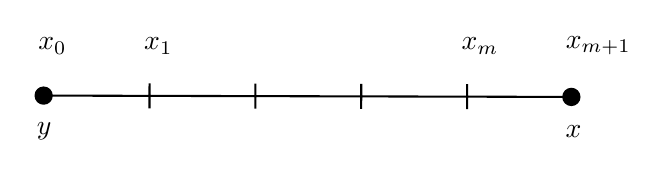
\begin{tikzpicture}[x=0.75pt,y=0.75pt,yscale=-1.5,xscale=1.5]
%uncomment if require: \path (0,68.99998474121094); %set diagram left start at 0, and has height of 68.99998474121094

%Straight Lines [id:da38713666625893595] 
\draw    (233.5,39) -- (403,39.43) (267.51,35.09) -- (267.49,43.09)(301.51,35.17) -- (301.49,43.17)(335.51,35.26) -- (335.49,43.26)(369.51,35.34) -- (369.49,43.34) ;


%Shape: Circle [id:dp053632030794002805] 
\draw  [fill={rgb, 255:red, 0; green, 0; blue, 0 }  ,fill opacity=1 ] (230.9,39) .. controls (230.9,37.56) and (232.06,36.4) .. (233.5,36.4) .. controls (234.94,36.4) and (236.1,37.56) .. (236.1,39) .. controls (236.1,40.44) and (234.94,41.6) .. (233.5,41.6) .. controls (232.06,41.6) and (230.9,40.44) .. (230.9,39) -- cycle ;
%Shape: Circle [id:dp6730801146643859] 
\draw  [fill={rgb, 255:red, 0; green, 0; blue, 0 }  ,fill opacity=1 ] (400.4,39.43) .. controls (400.4,37.99) and (401.56,36.82) .. (403,36.82) .. controls (404.44,36.82) and (405.6,37.99) .. (405.6,39.43) .. controls (405.6,40.87) and (404.44,42.03) .. (403,42.03) .. controls (401.56,42.03) and (400.4,40.87) .. (400.4,39.43) -- cycle ;

% Text Node
\draw (233.67,50.43) node   {$y$};
% Text Node
\draw (236.33,23.1) node   {$x_{0}$};
% Text Node
\draw (270.33,23.1) node   {$x_{1}$};
% Text Node
\draw (403.67,50.43) node   {$x$};
% Text Node
\draw (373.67,23.1) node   {$x_{m}$};
% Text Node
\draw (411.67,23.1) node   {$x_{m+1}$};


\end{tikzpicture}

					\end{center}
					\caption{Unterteilung des Intervalls $[y, x]$}
					\label{fig:Intervallunterteilung}
				\end{figure}
				

				Wähle $ m \in \N$ beliebig, definiere
				\begin{align*}
					t_{k}&:= \frac{k}{m+1} \text{ für } k=0, \ldots, m+1 \\
					x_{k}&:= y + t_{k}(x-y)
				\end{align*}
				Der Mittelwertsatz impliziert $\forall k=0, \ldots, m$ existiert ein $c_{k} \in(t_{k}, t_{k+1})$:
				\[
					f(x_{k+1}) -f(x_{k}) = \nabla  f(y + c_{k}(x-y))^{T}\underbrace{x_{k+1}- x_{k}}_{= (t_{k+1}- t_{k})(x-y)} 
				.\] 
				Damit folgt:
				\begin{align*}
					f(x)-f(y) &= f(x_{m+1}) - f(x_{0}) \\
							  &= \sum_{k=0}^{m}{f(x_{k+1}) - f(x_{k})} \\
							  &= \sum_{k=0}^{m}{(t_{k+1}-t_{k})\nabla f(y+c_{k}(x-y))^{T}(x-y)} \\
							  & \quad + \sum_{k=0}^{m}{(\nabla f(y) - \nabla f(x))^{T}\underbrace{t_{k+1}-t_{k})(x-y)}_{= x_{k+1}-x_{k}}} \\
							  &= \nabla f(y)^{T}(x-y) \\
							  & \quad + \sum_{k=0}^{m}{(t_{k+1}-t_{k})\left[ \nabla f(y+c_{k}(x-y)) - \nabla f(y) \right] ^{T} \underbrace{(x-y)}_{=\frac{1}{c_{k}}\left[ y + c_{k}(x-y) - y \right] } } \\
							  &\geq \nabla f(y)^{T}(x-y) \\
							  & \quad+ \sum_{k=0}^{m}{\frac{t_{k+1}- t_{k}}{c_{k}} \mu c_{k}^2 \norm{x-y} _{2}^2} \\
							  &= \nabla f(y)^{T}(x-y) + \frac{\mu \norm{x-y} _{2}}{m+1} \underbrace{\sum_{k=0}^{m}{\underbrace{c_{k}}_{\geq t_{k}= \frac{k}{m+1}} }}_{\geq \frac{m}{2}}   \\
							  &\geq \nabla f(y)^{T}(x-y) + \mu  \norm{x-y} ^2 \cdot \underbrace{\frac{m}{2(m+1)}}_{\rightarrow \frac{1}{2} \text{ für } m \rightarrow \infty} 
				\end{align*}
		\end{itemize}

\item (a): funktioniert wie (c) mit $\mu =0$ und ohne Intervallaufteilung. 
\item (b): funktioniert wie (c) mit $\mu =0$ mit strikten Ungleichungen und ohne Intervallaufteilung.
\end{itemize}
\end{proof}

\begin{satz}
\label{thm:monotonefunktionenunddefinitheit}
	Sei $X \subseteq \R^{n}$ nichtleer, affin, konvex und $F \colon X \rightarrow \R^{n} $ stetig diffbar. Dann gilt:
	\begin{enumerate}[label=(\alph{enumi})]
		\item $F$ monoton $\iff$ $\forall x \in X$ : $F(x)$ positiv semidefinit, d.h.
			\[
				d^{T}F'(x)d \geq 0 \quad \forall d \in \R^{n}
			.\] 
		\item $F$ strikt monoton $\Longleftarrow$ $\forall x \in X$ : $F'(x)$ ist positiv definit, d.h.
			\[
				d^{T}F'(x)d >  \quad \forall d \in \R^{n}\setminus \left\{ 0 \right\} 
			.\] 
		\item $F$ glm. monoton $\iff$ $\exists \mu > 0 ~ \forall x \in X$ : $F'$ glm. positiv definit
			\[
				d^{T} F'(x) d \geq \mu \norm{d} ^2 \quad \forall d \in \R^{n}
			.\]
	\end{enumerate}
\end{satz}

\begin{proof}
\label{thm:monotonefunktionenunddefinitheitbeweis}
\begin{itemize}
	\item (c)
		\begin{itemize}
			\item "$\implies$" : Sei $F$ glm. monoton, d.h. $\exists \mu > 0$ sodass $\forall x,y \in X$ : 
				\[
				(F(x)-F(y))^{T}(x-y) \geq \mu \norm{x-y} _{2}^2
				.\] 
				Sei $x \in X, d \in \R^{n}$ beliebig. Dann gilt
				\begin{align*}
					d^{T} \underbrace{F'(x)d}_{=F'(x;d)} &= \lim_{t \downarrow 0}  \frac{td^{T}(F(x+td) - F(x))}{t^2} \\
														 &\geq \lim_{t \downarrow 0}  \frac{\mu  t^2 \norm{d} ^2}{t^2} = \mu  \norm{d} ^2
				\end{align*}
				Das bedeutet $F'$ ist glm. positiv definit.

			\item "$\Longleftarrow$" : Sei $F'$ glm. positiv definit, d.h. $\exists \mu >0$ sodass $\forall x \in X ~ \forall d \in \R^{n}$ : 
				\[
					d^{T}F'(x)d \geq \mu \norm{d} _{2}^2
				.\] 
				Seien $x,y \in X$ beliebig. Dann gilt
				\begin{align*}
					(F(x)-F(y))^{T}(x-y) &= \int_{0}^{1} \underbrace{(x-y)^{T}F'(y+ \tau (x-y))(x-y)}_{\geq \mu \norm{x-y} _{2}^2} \d \tau \\
										 &\geq \mu  \norm{x-y} _{2}^2
				\end{align*}
		\end{itemize}
	\item (a) funktioniert wie (c) mit $\mu =0$
	\item (c) "$\Longleftarrow$" wie (c) mit $\mu =0$ und $F'$ positiv definit

		["$\implies$" geht kaputt wegen $\lim\limits_{t \downarrow 0}$ ]
\end{itemize}
\end{proof}

\begin{folgerung}
	Das folgende Diagramm zeigt alle bis zum jetzigen Zeitpunkt gezeigten Implikationen und Äquivalenzen.

\label{thm:monotonefunktionenkonvexefunktionenfolgerung}
\begin{figure}[H]
	\begin{center}
		

\tikzset{every picture/.style={line width=0.75pt}} %set default line width to 0.75pt        

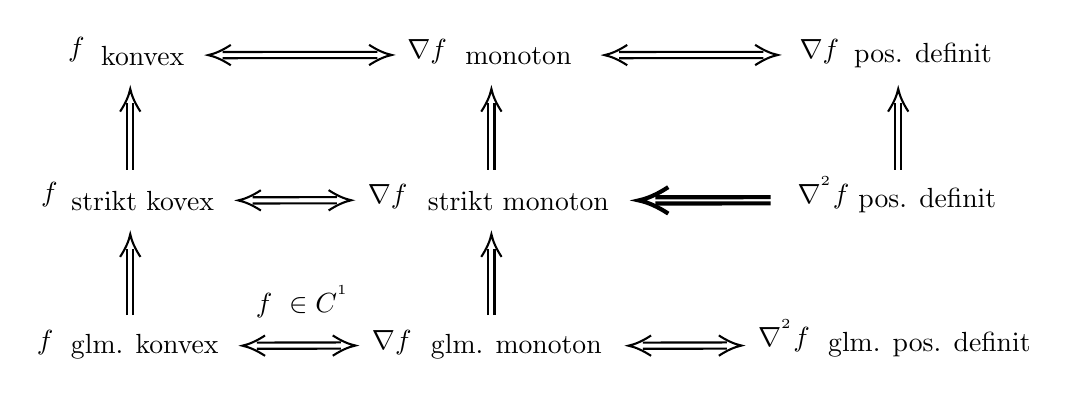
\begin{tikzpicture}[x=0.75pt,y=0.75pt,yscale=-1,xscale=1]
%uncomment if require: \path (0,184.43749237060547); %set diagram left start at 0, and has height of 184.43749237060547




%Straight Lines [id:da6931552921369328] 
\draw [line width=0.75]    (502.5,79.01) -- (502.5,47.01)(505.5,79.01) -- (505.5,47.01) ;
\draw [shift={(504,40.01)}, rotate = 450] [color={rgb, 255:red, 0; green, 0; blue, 0 }  ][line width=0.75]    (10.93,-4.9) .. controls (6.95,-2.3) and (3.31,-0.67) .. (0,0) .. controls (3.31,0.67) and (6.95,2.3) .. (10.93,4.9)   ;




%Straight Lines [id:da5376916843087101] 
\draw [line width=0.75]    (306.5,79.01) -- (306.5,47.01)(309.5,79.01) -- (309.5,47.01) ;
\draw [shift={(308,40.01)}, rotate = 450] [color={rgb, 255:red, 0; green, 0; blue, 0 }  ][line width=0.75]    (10.93,-4.9) .. controls (6.95,-2.3) and (3.31,-0.67) .. (0,0) .. controls (3.31,0.67) and (6.95,2.3) .. (10.93,4.9)   ;

%Straight Lines [id:da9601126151289101] 
\draw [line width=0.75]    (306.5,149.01) -- (306.5,117.01)(309.5,149.01) -- (309.5,117.01) ;
\draw [shift={(308,110.01)}, rotate = 450] [color={rgb, 255:red, 0; green, 0; blue, 0 }  ][line width=0.75]    (10.93,-4.9) .. controls (6.95,-2.3) and (3.31,-0.67) .. (0,0) .. controls (3.31,0.67) and (6.95,2.3) .. (10.93,4.9)   ;





%Straight Lines [id:da17111805237135647] 
\draw [line width=0.75]    (132.5,79.01) -- (132.5,47.01)(135.5,79.01) -- (135.5,47.01) ;
\draw [shift={(134,40.01)}, rotate = 450] [color={rgb, 255:red, 0; green, 0; blue, 0 }  ][line width=0.75]    (10.93,-4.9) .. controls (6.95,-2.3) and (3.31,-0.67) .. (0,0) .. controls (3.31,0.67) and (6.95,2.3) .. (10.93,4.9)   ;

%Straight Lines [id:da6402722120192785] 
\draw [line width=0.75]    (132.5,149.01) -- (132.5,117.01)(135.5,149.01) -- (135.5,117.01) ;
\draw [shift={(134,110.01)}, rotate = 450] [color={rgb, 255:red, 0; green, 0; blue, 0 }  ][line width=0.75]    (10.93,-4.9) .. controls (6.95,-2.3) and (3.31,-0.67) .. (0,0) .. controls (3.31,0.67) and (6.95,2.3) .. (10.93,4.9)   ;


%Straight Lines [id:da19646642044249396] 
\draw [line width=1.5]    (442.5,95.15) -- (387,95.21)(442.5,92.15) -- (387,92.21) ;
\draw [shift={(379,93.72)}, rotate = 359.93] [color={rgb, 255:red, 0; green, 0; blue, 0 }  ][line width=1.5]    (14.21,-6.37) .. controls (9.04,-2.99) and (4.3,-0.87) .. (0,0) .. controls (4.3,0.87) and (9.04,2.99) .. (14.21,6.37)   ;

%Straight Lines [id:da012310767209407603] 
\draw [line width=0.75]    (439,25.15) -- (369.5,25.22)(439,22.15) -- (369.5,22.22) ;
\draw [shift={(362.5,23.72)}, rotate = 359.95] [color={rgb, 255:red, 0; green, 0; blue, 0 }  ][line width=0.75]    (10.93,-4.9) .. controls (6.95,-2.3) and (3.31,-0.67) .. (0,0) .. controls (3.31,0.67) and (6.95,2.3) .. (10.93,4.9)   ;
\draw [shift={(446,23.65)}, rotate = 179.95] [color={rgb, 255:red, 0; green, 0; blue, 0 }  ][line width=0.75]    (10.93,-4.9) .. controls (6.95,-2.3) and (3.31,-0.67) .. (0,0) .. controls (3.31,0.67) and (6.95,2.3) .. (10.93,4.9)   ;
%Straight Lines [id:da8068390743979135] 
\draw [line width=0.75]    (421.5,165.16) -- (381,165.21)(421.5,162.16) -- (381,162.21) ;
\draw [shift={(374,163.72)}, rotate = 359.91999999999996] [color={rgb, 255:red, 0; green, 0; blue, 0 }  ][line width=0.75]    (10.93,-4.9) .. controls (6.95,-2.3) and (3.31,-0.67) .. (0,0) .. controls (3.31,0.67) and (6.95,2.3) .. (10.93,4.9)   ;
\draw [shift={(428.5,163.65)}, rotate = 179.92] [color={rgb, 255:red, 0; green, 0; blue, 0 }  ][line width=0.75]    (10.93,-4.9) .. controls (6.95,-2.3) and (3.31,-0.67) .. (0,0) .. controls (3.31,0.67) and (6.95,2.3) .. (10.93,4.9)   ;
%Straight Lines [id:da7137872354673338] 
\draw [line width=0.75]    (235.5,165.16) -- (195,165.21)(235.5,162.16) -- (195,162.21) ;
\draw [shift={(188,163.72)}, rotate = 359.91999999999996] [color={rgb, 255:red, 0; green, 0; blue, 0 }  ][line width=0.75]    (10.93,-4.9) .. controls (6.95,-2.3) and (3.31,-0.67) .. (0,0) .. controls (3.31,0.67) and (6.95,2.3) .. (10.93,4.9)   ;
\draw [shift={(242.5,163.65)}, rotate = 179.92] [color={rgb, 255:red, 0; green, 0; blue, 0 }  ][line width=0.75]    (10.93,-4.9) .. controls (6.95,-2.3) and (3.31,-0.67) .. (0,0) .. controls (3.31,0.67) and (6.95,2.3) .. (10.93,4.9)   ;
%Straight Lines [id:da3667450709373552] 
\draw [line width=0.75]    (233.5,95.16) -- (193,95.21)(233.5,92.16) -- (193,92.21) ;
\draw [shift={(186,93.72)}, rotate = 359.91999999999996] [color={rgb, 255:red, 0; green, 0; blue, 0 }  ][line width=0.75]    (10.93,-4.9) .. controls (6.95,-2.3) and (3.31,-0.67) .. (0,0) .. controls (3.31,0.67) and (6.95,2.3) .. (10.93,4.9)   ;
\draw [shift={(240.5,93.65)}, rotate = 179.92] [color={rgb, 255:red, 0; green, 0; blue, 0 }  ][line width=0.75]    (10.93,-4.9) .. controls (6.95,-2.3) and (3.31,-0.67) .. (0,0) .. controls (3.31,0.67) and (6.95,2.3) .. (10.93,4.9)   ;
%Straight Lines [id:da16014383432778323] 
\draw [line width=0.75]    (253,25.15) -- (178.5,25.22)(253,22.15) -- (178.5,22.22) ;
\draw [shift={(171.5,23.72)}, rotate = 359.95] [color={rgb, 255:red, 0; green, 0; blue, 0 }  ][line width=0.75]    (10.93,-4.9) .. controls (6.95,-2.3) and (3.31,-0.67) .. (0,0) .. controls (3.31,0.67) and (6.95,2.3) .. (10.93,4.9)   ;
\draw [shift={(260,23.65)}, rotate = 179.95] [color={rgb, 255:red, 0; green, 0; blue, 0 }  ][line width=0.75]    (10.93,-4.9) .. controls (6.95,-2.3) and (3.31,-0.67) .. (0,0) .. controls (3.31,0.67) and (6.95,2.3) .. (10.93,4.9)   ;


% Text Node
\draw (108,20.87) node   {$f$};
% Text Node
\draw (140,23.87) node  [align=left] {konvex};
% Text Node
\draw (277,22) node   {$\nabla f$};
% Text Node
\draw (321,24) node  [align=left] {monoton};
% Text Node
\draw (466,22) node   {$\nabla f$};
% Text Node
\draw (516,24) node  [align=left] {pos. definit};
% Text Node
\draw (95,91) node   {$f$};
% Text Node
\draw (140,94) node  [align=left] {strikt kovex};
% Text Node
\draw (258,92) node   {$\nabla f$};
% Text Node
\draw (321,94) node  [align=left] {strikt monoton};
% Text Node
\draw (468,90) node   {$\nabla ^{^{2}} f$};
% Text Node
\draw (518,94) node  [align=left] {pos. definit};
% Text Node
\draw (93,162) node   {$f$};
% Text Node
\draw (141,164) node  [align=left] {glm. konvex};
% Text Node
\draw (260,162) node   {$\nabla f$};
% Text Node
\draw (320,164) node  [align=left] {glm. monoton};
% Text Node
\draw (449,159) node   {$\nabla ^{^{2}} f$};
% Text Node
\draw (519,163) node  [align=left] {glm. pos. definit};
% Text Node
\draw (217,142.44) node   {$f\ \in C^{^{1}}$};


\end{tikzpicture}

	\end{center}
	\caption{Zusammenfassung aller Äquivalenzen und Folgerungen}
	\label{fig:ZusammenfassungKonvexUndMonoton}
\end{figure}

\end{folgerung}

\begin{definition}
\label{thm:pseudoquasimonoton}
	Sei $X \subseteq \R^{n}$ und $F \colon X \rightarrow \R^{n} $
	\begin{enumerate}[label=(\alph{enumi})]
		\item  $F$ heißt \underline{pseudomonoton} $\iff$ $\forall x,y \in X$ : 
			\[
				F(y)^{T}(x-y) \geq 0 \implies F(x)^{T}(x-y) \geq 0
			.\] 
		\item $F$ heißt \underline{quasimonoton} $\iff$ $\forall x,y \in X$ :
			\[
				\min \left\{ F(x)^{T}(x-y), F(y)^{T}(y-x) \right\} \leq 0
			.\] 
	\end{enumerate}

	Man kann zeigen:
	\begin{itemize}
		\item $f$ pseudokonvex $\iff$ $\nabla f$ pseudomonoton
		\item Ist $F$ pseudomonoton, so gilt $\forall x,y \in X$ :
			\[
				F(y)^{T} (x-y) > 0 \implies F(x)^{T} (x-y) > 0
			.\] 
		\item Ist $F$ quasimonoton und diffbar, so ist $\nabla F$ quasimonoton
	\end{itemize}
\end{definition}

\section{Grundlagen aus der nichtlinearen Optimierung}%
\label{sec:Grundlagen aus der nichtlinearen Optimierung}

Optimierungsproblem: 
\[
 \min\limits_{x} f(x) \text{ udN } x \in X
.\]
("udN" $\stackeq{\wedge}$ unter der Nebenbedingung)

mit
\begin{itemize}
	\item Variablen $x \in \R^{n}$
	\item Zielfunktion $f \colon X \rightarrow \R $ (gegebenenfalls auf offener Obermenge von $X$ definiert)
	\item zulässige Menge $X \subseteq \R^{n}$ 

		(oft: $X = \left\{ x \in \R^{n} | g(x) \leq 0, h(x) = 0 \right\} $ mit $g \colon \R^{n} \rightarrow \R^{m}, h \colon \R^{n} \rightarrow \R^{p}$)
\end{itemize}

In dieser Vorlesung gilt meistens
\begin{itemize}
	\item $X \subseteq \R^{n}$ nichtleer, abgeschlossen, konvex
	\item $f$ konvex und stetig diffbar
\end{itemize}

\begin{satz}[Minimierungsprinzip]
\label{thm:minimierungsprinzip}
	Sei $X \subseteq \R^{n}$ nichtleer, konvex und $f \colon X \rightarrow \R $ stetig diffbar. Dann gelten
	\begin{enumerate}[label=(\alph{enumi})]
		\item Ist $x^{*}\in X$ ein lokales Minimum von $f$ auf $X$, so gilt
			\[
				\nabla f(x^{*})^{T}(x-x^{*}) \geq 0 \quad \forall x \in X
			.\] 
		\item Ist $f$ pseudokonvex und gilt $\nabla f(x^{*})^{T}(x-x^{*})\geq 0$ für alle $x \in X$, so ist $x^{*}$ ein \underline{globales} Minimum von $f$ auf $X$
	\end{enumerate}
\end{satz}

\begin{proof}
\label{thm:minimierungsprinzipbeweis}
\begin{itemize}
	\item (b) Aus der Definition von Pseudokonvexität folgt $f(x) \geq f(x^{*})\quad \forall x \in X$.
	\item (a) Sei $x^{*}$ ein lokales Minimum von $f$ auf $X$. Angenommen, es gibt $x \in X$ mit
		\[
			f'(x^{*}; x- x^{*}) = \nabla f(x^{*})^{T}(x-x^{*}) < 0
		.\] 
		Dann ist $x-x^{*}$ eine Abstiegsrichtung, denn es gilt
		\[
			0 > f'(x^{*};x-x^{*}) = \lim_{t \downarrow 0} \frac{f(x^{*} + t(x-x^{*}))-f(x^{*})}{t}
		.\] 
		\[
			\implies \forall t > 0 \text{ (klein) }: f(\underbrace{x^{*}+t(x-x^{*})}_{\substack{\in X, \text{ da $X$ konvex }\\ \rightarrow x^{*} \text{ für } t \downarrow 0}} ) < f(x^{*})
		.\] 
		$\lightning$ $x^{*}$ lokales Minimum.
\end{itemize}
\end{proof}

\begin{itemize}
	\item Fall $X$ konvex: $x^{*}$ lokales Minimum $\implies$ $f'(x^{*};d)\geq 0$ für alle zulässigen Richtungen $d=x-x^{*}$ mit $x \in X$.
	\item Fall $X$ beliebig: $x^{*}$ lokales Minimum $\implies$ $f'(x^{*};d)\geq 0$ für alle "zulässigen" Richtungen $d$. Was bedeutet "zulässig" in diesem Fall?

		$\implies$ Bouligand-Tangentialkegel:
		\[
			T_{X}(x^{*}):= \left\{ d \in \R^{n} ~|~ \exists (x^{k})_{k} \subseteq X \text{ und } (t_{k})_{k}\geq 0 ~\colon x^{k} \rightarrow x^{*} \text{ und } t_{k}(x^{k}-x^{*}) \rightarrow d \right\} 
		.\] ($t_{k}$ ist hierbei oft definiert durch $t_{k}=\frac{1}{\norm{x^{k}- x^{*}} }$)
\end{itemize}

\begin{satz}
\label{thm:lokalesminimumsatz}
	Sei $x^{*}$ lokales Minimum von $f$ auf $X$
	\[
		\implies \nabla f(x^{*})^{T}d \geq 0 \quad \forall d \in T_{X}(x^{*})
	.\] 
	(ohne Beweis)
\end{satz}

\underline{Problem}:

$T_{X}(x^{*})$ ist im Allgemeinen schwer zu berechnen. Deshalb verwende den \underline{Linearisierungskegel} an $X=\left\{ x ~|~ g(x) \leq 0, h(x) = 0 \right\}$ in $x^{*}$:
\begin{align*}
	L_{X}(x^{*}) &= \left\{ d \in \R^{n} ~|~ \nabla g_{i}(x^{*})^{T}d \leq 0 \quad \forall i \in Ig(x^{*})= \left\{ i ~|~ g_{i}(x^{*}) = 0\right\}\right\}\\
				 &\qquad\cap \left\{ d \in \R^{n} ~|~ \nabla h_{i}(x^{*})^{T}d = 0 \quad \forall i=1, \ldots, p \right\} \\
				 &= T_{X_{\text{lin}}}(x^{*})
\end{align*}
Sei $x^{*} \in X$, definiere
\begin{align*}
	X_{\text{lin}}=&\left\{ x \in \R^{n} ~|~ g(x^{*}) + \nabla  g(x^{*})^{T}(x-x^{*}) \leq 0\right\} \\
	&\qquad\cap \left\{ x \in \R^{n} ~|~ h(x^{*}) + \nabla h(x^{*})^{T}(x-x^{*}) = 0 \right\} 
\end{align*}

\begin{itemize}
	\item Es gilt immer $T_{X}(x^{*}) \subseteq L_{X}(x^{*})$
	\item Es gilt 
		\[
		\nabla f(x^{*})d \geq 0 \quad \forall d \in L_{X}(x^{*})
		,\] genau dann, wenn es Multiplikatoren $Z \in \R^{m}$ und $\mu \in \R^{p}$ gibt mit
		\[
		\left.
		\begin{array}{r}
			\nabla f(x^{*}) + \sum_{i=1}^{m}Z_{i}\nabla g_{i}(x^{*}) + \sum_{i=1}^{p}\mu _{i}\nabla h_{i}(x^{*})=0 \\
			h(x^{*}) = 0 \\
			\forall i=1, \ldots, m \colon g_{i}(x^{*})\leq 0 \leq Z_{i} \text{ mit } Z_{i}\cdot g_{i}(x^{*}) = 0
		\end{array}
		\right] \text{ KKT-Bedingungen }
		.\] 
		Es gilt folgende nützlich Implikation
		\begin{align*}
			x^{*} \text{ lokales Minimum } &\implies \nabla f(x^{*})^{T}d \geq 0 \forall d \in T_{X}(x^{*}) \subseteq L_{X}(x^{*}) \\
			\overset{(\ast)}&{\iff}  \nabla f(x^{*})^{T}d \geq 0 \forall d \in L_{X}(x^{*}) \\
										   &\iff x^{*} \text{ ist ein KKT-Punkt }
		\end{align*}
		Die Äquivalenz $(\ast)$ gilt hierbei nur unter der sogenannten "constraint qualification" (CQ), die garantiert, dass $T_{X}(x^{*}) = L_{X}(x^{*})$ gilt.
\end{itemize}

Beispiele für Constraint Qualifications:
\begin{itemize}
	\item Abadie-CQ :
		\[
		T_{X}(x^{*})=L_{X}({x}^{*})
		.\] 
	\item Linear Independence CQ (LICQ): 
		\begin{align*}
			&\nabla h_{i}({x}^{*}) \quad (i=1, \ldots, p) \\ 
			&\nabla g_{i}({x}^{*})\quad (i \in Ig({x}^{*}) )
		\end{align*}
		  sind linear unabhängig.
	\item Mangasarian-Fromowitz-CQ (MFCQ):

		Es gilt
		\begin{itemize}
			\item $\nabla h_{i}({x}^{*})$ $(i=1, \ldots, p)$ sind linear unabhängig
			\item $\exists d \in \R^{n}$:
				\begin{align*}
				&\nabla g_{i}({x}^{*})^{T}d < 0 \quad \forall i \in Ig({x}^{*}) \\
				&\nabla h_{i}({x}^{*})=0\quad \forall i=1, \ldots, p
				\end{align*}
		\end{itemize}
	\item Linearitäts-CQ:

		Die Funktionen $g(x)$ und $h(x)$ sind linear.
	\item Slater-CQ:

		Für konvexe Mengen $X$, d.h. $g_{i}$ konvex $\forall i=1, \ldots, m$, $h$ affin linear:

		\[
			\text{ Es gibt ein } \hat{x} \in X \text{ mit } g(\hat{x}) < 0
		.\] 
\end{itemize}

\begin{satz}
\label{thm:optinumsatzletzter}
\begin{enumerate}[label=(\alph{enumi})]
	\item ${x}^{*}$ lokales Minimum + CQ in ${x}^{*}$ $\implies$ ${x}^{*}$ ist ein KKT-Punkt
	\item ${x}^{*}$ KKT-Punkt + $f$, $g_{i}$ konvex, $h$ affin linear $\implies$ ${x}^{*}$ ist ein globales Minimum
\end{enumerate}
\end{satz}

Problemklassen und mögliche Lösungsalgorithmen

\begin{itemize}
	\item lineare Probleme:
		\[
		\min\limits_{x}c^{T}x \qquad\text{ udN } Ax=b, x \geq 0
		.\] 
		Löse zum Beispiel mit Simplex-Verfahren oder Innere-Punkte-Verfahren.
	\item quadratische Probleme:
		\[
			\min\limits_{x}\frac{1}{2}x^{T}Qx + q^{T}x + \gamma \qquad\text{ udN } Ax=b, x\geq 0
		.\] 
		Löse zum Beispiel mit der Strategie der aktiven Menge.
	\item unrestringierte Probleme:
		\[
			\min\limits_{\lambda \in \R^{n}}f(x)
		.\] 
		Löse zum Beispiel mit Gradientenverfahren, Newton-Verfahren oder Trust-Region-Verfahren.
	\item restringierte Probleme:
		\[
			\min\limits_{x} f(x) \qquad\text{ udN } g(x) \leq 0 \text{ und } h(x) = 0
		.\] 
		Löse zum Beispiel mit Penalty-Verfahren, Barriere-Verfahren oder SQP-Verfahren.
	\item lineare Komplementaritätsprobleme:
		\[
			\text{ Finde }x \in \R^{n} \text{ mit } x \geq 0, Mx+q \geq 0 \text{ und }x^{T}(Mx+q) = 0
		.\] 
		Löse zum Beispiel mit Lemke-Verfahren
\end{itemize}

\section{Projektionen}%
\label{sec:Projektionen}

Fragestellung: gegeben $X \subseteq \R^{n}$, $y \not \in X$, finde "beste Approximation" von $y$ in $X$.

\begin{definition}
\label{thm:euklidischenorm}
	Die \underline{euklidische Norm} ist definiert durch
	\[
	\norm{x} _{2}:= \sqrt{x^{T}x}  
	.\] 
	Die \underline{gewichtete euklidische Norm} ist definiert durch
	\[
	\norm{x} _{G}:= \sqrt{x^{T}Gx} 
	.\] 
	(Mit $G \in \R^{n \times n}$ symmetrisch positiv definit)
\end{definition}

\begin{satz}[Projektionen]
\label{thm:projektionssatz}
	\begin{enumerate}[label=(\alph{enumi})]
		\item Sei $X \subseteq \R^{n}$ nichtleer, abgeschlossen, konvex, $y \not \in X$, $G \in \R^{n \times n}$ s.p.d. Dann hat das Problem 
		\[
		\min\limits_{x}\norm{y-x} _{G} \text{ udN } x \in X
		\] 
		genau eine Lösung ${x}^{*}$. Man sagt ${x}^{*}=P_{X,G}(y)$ ist die \underline{Projektion} von $y$ auf $X$ (bezüglich der Norm $\norm{\cdot} _{G}$).
		\item Es gilt: ${x}^{*} \in X$ ist die Projektion von $y$ auf $X$ genau dann, wenn
			\[
				\forall x \in X: \quad (y-{x}^{*})^{T}G(x-{x}^{*}) \leq 0
			.\] 
			\begin{figure}[H]
				\begin{center}
					

\tikzset{every picture/.style={line width=0.75pt}} %set default line width to 0.75pt        

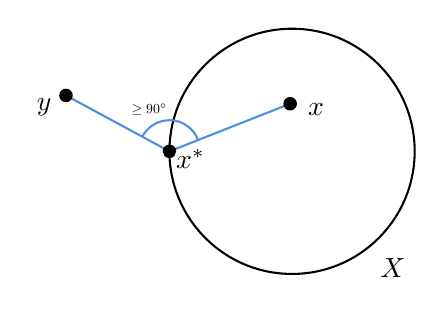
\begin{tikzpicture}[x=0.75pt,y=0.75pt,yscale=-1,xscale=1]
%uncomment if require: \path (0,159.1517791748047); %set diagram left start at 0, and has height of 159.1517791748047

%Shape: Circle [id:dp793276566783315] 
\draw  [color={rgb, 255:red, 0; green, 0; blue, 0 }  ,draw opacity=1 ] (304.85,79.08) .. controls (304.85,46.45) and (331.3,20) .. (363.92,20) .. controls (396.55,20) and (423,46.45) .. (423,79.08) .. controls (423,111.7) and (396.55,138.15) .. (363.92,138.15) .. controls (331.3,138.15) and (304.85,111.7) .. (304.85,79.08) -- cycle ;
%Straight Lines [id:da7340499227951829] 
\draw [color={rgb, 255:red, 74; green, 144; blue, 226 }  ,draw opacity=1 ]   (255,52.15) -- (304.85,79.08) -- (363,56.15) ;


%Shape: Circle [id:dp5288970197229892] 
\draw  [fill={rgb, 255:red, 0; green, 0; blue, 0 }  ,fill opacity=1 ] (252.25,52.15) .. controls (252.25,50.63) and (253.48,49.4) .. (255,49.4) .. controls (256.52,49.4) and (257.75,50.63) .. (257.75,52.15) .. controls (257.75,53.67) and (256.52,54.9) .. (255,54.9) .. controls (253.48,54.9) and (252.25,53.67) .. (252.25,52.15) -- cycle ;
%Shape: Circle [id:dp8279885137504637] 
\draw  [fill={rgb, 255:red, 0; green, 0; blue, 0 }  ,fill opacity=1 ] (302.1,79.08) .. controls (302.1,77.56) and (303.33,76.33) .. (304.85,76.33) .. controls (306.37,76.33) and (307.6,77.56) .. (307.6,79.08) .. controls (307.6,80.59) and (306.37,81.83) .. (304.85,81.83) .. controls (303.33,81.83) and (302.1,80.59) .. (302.1,79.08) -- cycle ;
%Shape: Circle [id:dp1357970650709539] 
\draw  [fill={rgb, 255:red, 0; green, 0; blue, 0 }  ,fill opacity=1 ] (360.25,56.15) .. controls (360.25,54.63) and (361.48,53.4) .. (363,53.4) .. controls (364.52,53.4) and (365.75,54.63) .. (365.75,56.15) .. controls (365.75,57.67) and (364.52,58.9) .. (363,58.9) .. controls (361.48,58.9) and (360.25,57.67) .. (360.25,56.15) -- cycle ;
%Shape: Arc [id:dp4881996475338144] 
\draw  [draw opacity=0] (291.71,72.11) .. controls (294.19,67.33) and (299.14,64.08) .. (304.85,64.08) .. controls (311.1,64.08) and (316.46,68) .. (318.63,73.54) -- (304.85,79.08) -- cycle ; \draw  [color={rgb, 255:red, 74; green, 144; blue, 226 }  ,draw opacity=1 ] (291.71,72.11) .. controls (294.19,67.33) and (299.14,64.08) .. (304.85,64.08) .. controls (311.1,64.08) and (316.46,68) .. (318.63,73.54) ;


% Text Node
\draw (244.5,58) node   {$y$};
% Text Node
\draw (375.5,59) node   {$x$};
% Text Node
\draw (315,83) node   {$x^{\ast }$};
% Text Node
\draw (412.5,135.5) node   {$X$};
% Text Node
\draw (295,59) node [scale=0.5]  {$\geq 90^{\circ} $};


\end{tikzpicture}

				\end{center}
				\caption{Veranschaulichung von (b)}
				\label{fig:projektionssatzbild}
			\end{figure}
			
		\item Die Abbildung $y \mapsto P_{X,G}(y)$ ist Lipschitz-stetig mit $L = 1$, insbesondere stetig.
	\end{enumerate}
\end{satz}

\begin{proof}
\label{thm:projektionssatzbeweis}
\begin{itemize}
	\item (a) sollte man kennen, ist ein Standardbeweis, siehe Funktionalanalysis "Projektionssatz"
	\item (b) 
		\begin{align*}
			{x}^{*}=P_{X,G}(y) &\iff {x}^{*} \text{ löst } \min\limits_{x}\underbrace{\norm{y-x} _{G}^2}_{=(y-x)^{T}G(y-x)=:f(x)}  \text{ udN } x \in X \\
			\overset{(\ast)}&{\iff}  \nabla f({x}^{*})^{T}(x-{x}^{*}) \geq 0 \quad \forall x \in X \\
							   &\iff -2 \left[ G(y-{x}^{*}) \right] ^{T} (x-{x}^{*}) \geq 0 \quad \forall x \in  X \\
							   &\iff (y-{x}^{*})^{T}G(x-{x}^{*}) \leq 0 \quad \forall x \in X
		\end{align*}
		$(\ast)$ Beachte hier, dass $X$ und $f$ konvex sind.
	\item (c) Seien $y,z \in \R^{n}$.
		\begin{align*}
			\implies y-z &= P_{X,G}(y) - P_{X,G}(z) + \underbrace{(y-P_{X,G}(y)) + (P_{X,G}(z) - z)}_{=:u}  \\
			\implies \norm{y-z} _{G}^2 &= \norm{P_{X,G}(y) -P_{X,G}(z)} _{G}^2 + \underbrace{\norm{u} _{G}^{2}}_{\geq 0}  + 2 (P_{X,G}(y) - P_{X,G}(z))^{T}Gu \\
									   & \geq  \norm{P_{X,G}(y) -P_{X,G}(z)} _{G}^2 + \underbrace{2 (P_{X,G}(y)-P_{X,G}(z))^{T}(y-P_{X,G}(y))}_{\geq 0}  \\
									   & \qquad \qquad \qquad \qquad \qquad \quad + \underbrace{2 (P_{X,G}(y)-P_{X,G}(z))^{T}(P_{X,G}(z)-z)}_{\geq 0}  \\
									   &\geq\norm{P_{X,G}(y) -P_{X,G}(z)} _{G}^2
		\end{align*}
		
\end{itemize}
\end{proof}
